\documentclass{scrartcl}
\usepackage{tabularx}
\usepackage{booktabs}
\usepackage{csquotes}
% Include Graphic-files:
\usepackage{graphicx}
\usepackage{caption}
\usepackage{subfig}
%\usepackage{subfig}
\newsubfloat{figure}
\newcommand{\source}[1]{\vspace{-3pt} \caption*{ Source: {#1}} }

\begin{document}

\begin{figure}[!t]
\centering
  \begin{minipage}{0.3\textwidth}
  \centering
  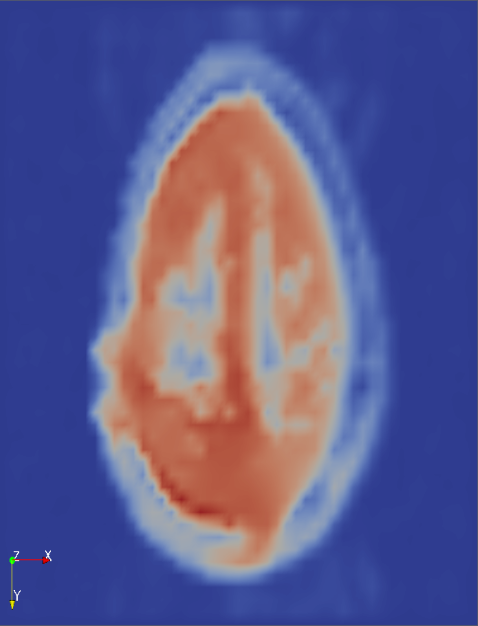
\includegraphics[width=\textwidth]{img_new/brain_surf.PNG}
     \label{a)}
      a)
  \end{minipage}
  \begin{minipage}{0.3\textwidth}
    \centering
    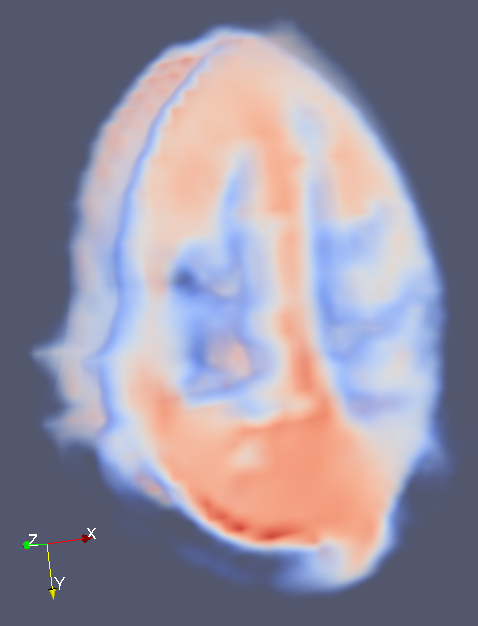
\includegraphics[width=\textwidth]{img_new/brain_volume2.PNG}
    \label{b)}
    b)
  \end{minipage}
  \begin{minipage}{0.3\textwidth}
    \centering
    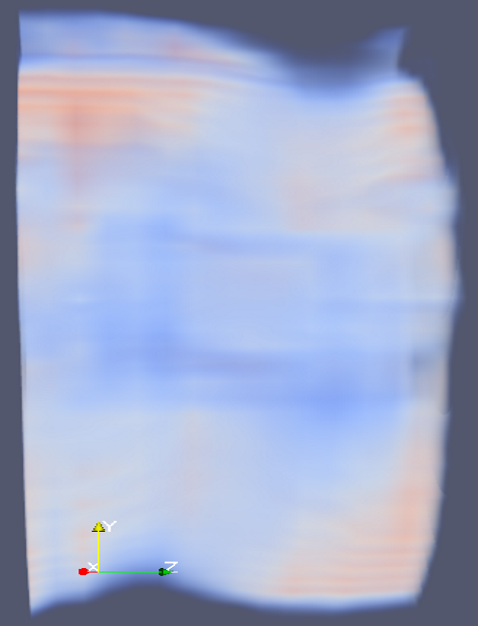
\includegraphics[width=\textwidth]{img_new/brain_cross-section.PNG}
    c)
    \label{b)}
  \end{minipage}
  \caption{\enquote{brain} test field: a) LTG($0^\circ$), b) LTG volume, c) cross-section}
\label{heart-ftle}
\end{figure}

\begin{figure}[!t]
\centering
  \begin{minipage}{0.3\textwidth}
  \centering
  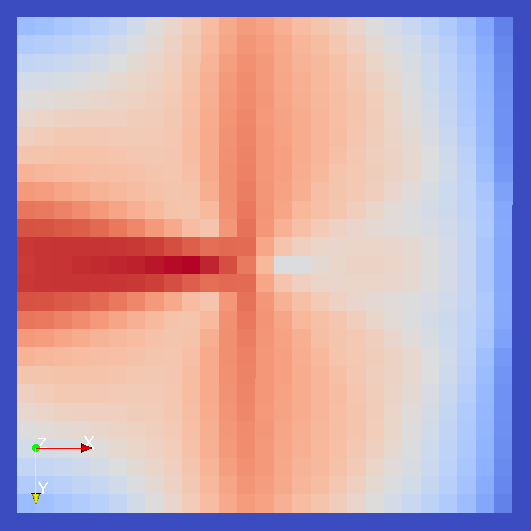
\includegraphics[height=\textwidth]{img/inverse29.png}\label{1a}
    a)
    \label{a)}
  \end{minipage}
  \begin{minipage}{0.3\textwidth}
  \centering
    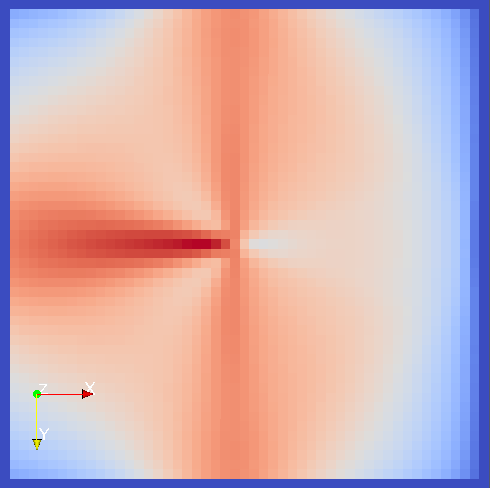
\includegraphics[height=\textwidth]{img/inverse51.PNG}\label{2a}
	b)
    \label{b)}
  \end{minipage}
  \begin{minipage}{0.3\textwidth}
  \centering
    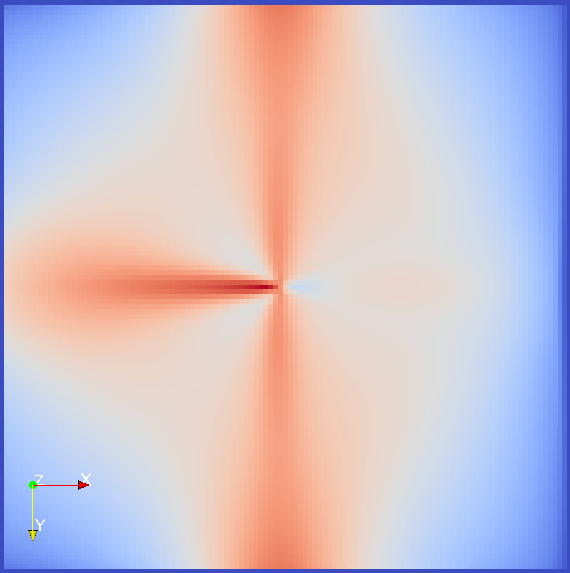
\includegraphics[height=\textwidth]{img/inverse101.PNG}
	c)
    \label{b)}
  \end{minipage}
  \caption{ \protect a) some text 
  \protect b) some other text}
\label{res_ftle}
\end{figure}
%%%%%%%%%%%%%%%%%%%%%%%%%%%%%%%%%%%%%%%%%%%%%%%%%%%%%%%%%%%%

% Alternative: put content in separate files
% Check the difference between including these files using \input{filename} and \include{filename} and see which one you like better
%\chapter{Einleitung}\label{intro}
%\input{introduction}
%
%\chapter{Voraussetzungen}\label{bg}
%\input{background}



\end{document}